\usepackage{booktabs}
\usepackage{listings}
\usepackage{tikz}%! Author = abenjeddou
%! Date = 30/06/2026

\chapter{Implementation}
\label{chap:implementation}

This chapter details the implementation of the \textbf{LFU (Limited Fair Use)} job within the \textit{Pushavoo-Flink} platform. The development was organized into \textbf{6 sprints}, following an Agile Scrum methodology with two-week iterations. Each sprint delivered a working increment of the system, from the initial project setup through to full observability in production.

Table~\ref{tab:sprint-overview} provides an overview of the sprint planning.

\begin{table}[H]
    \centering
    \caption{Sprint planning overview}
    \label{tab:sprint-overview}
    \begin{tabularx}{\textwidth}{c l X}
\toprule
\textbf{Sprint} & \textbf{Theme} & \textbf{Key Deliverables} \\
\midrule
1 & Project Setup \& Message Ingestion & Maven module, RabbitMQ source, message validation \\
2 & Subscription \& Business Rules & Valkey integration, main record retrieval, rule validation \\
3 & Notification Delivery & Erable API call, retry mechanism, state update sink \\
4 & AI Prediction Module & Feature extraction, ONNX inference, rule-based fallback \\
5 & Containerization \& Deployment & Docker image, Kubernetes, CI/CD pipeline \\
6 & Observability \& Monitoring & Structured logging, Kibana dashboards, Grafana metrics \\
\bottomrule
    \end{tabularx}
\end{table}

%######################################################################
%######################################################################
\section{Sprint 1: Project Setup and Message Ingestion}
\label{sec:sprint1}
%######################################################################
%######################################################################

\subsection{Sprint Goal}

Establish the project foundation and implement the first two pipeline operators: RabbitMQ message consumption and incoming message validation.

\subsection{Technology Stack}

\begin{table}[H]
    \centering
    \caption{LFU job technology stack}
    \label{tab:stack}
    \begin{tabularx}{\textwidth}{l l X}
\toprule
\textbf{Category} & \textbf{Technology} & \textbf{Version / Details} \\
\midrule
Language & Java & 17 (LTS) \\
Streaming Framework & Apache Flink & 1.20.2 \\
Build & Apache Maven & Shade plugin (fat JAR) \\
Message Broker & RabbitMQ & Flink Connector 3.0.1-1.17 \\
State Store & Valkey & REST API (Redis-compatible) \\
Notification API & Erable & HTTP/REST via Spring WebClient \\
AI Inference & ONNX Runtime & 1.17.0 \\
Serialization & Jackson & 2.15.2 \\
Validation & Hibernate Validator & 6.2.5.Final (Bean Validation 2.0) \\
Logging & Logback + Logstash encoder & 1.2.13 / 7.2 \\
Containerization & Docker & Based on Flink 1.20.1 image \\
Orchestration & Kubernetes / Docker Compose & High availability with ZooKeeper \\
Authentication & OKAPI v2 & OAuth2 token \\
\bottomrule
    \end{tabularx}
\end{table}

\subsection{Project Structure}

The \texttt{pushavoo-flink} project is organized into Maven modules:

\begin{itemize}
    \item \texttt{pushavoo-flink-core} --- Shared library (utilities, metrics, RabbitMQ connectors, Erable client, Valkey access)
    \item \texttt{pushavoo-flink-jobs/job-fair-use} --- The LFU job (subject of this report)
    \item \texttt{pushavoo-flink-jobs/job-fiber-eligibility} --- Fiber eligibility job
    \item \texttt{pushavoo-flink-jobs/job-contracts-portfolio-changes} --- Portfolio changes job
    \item \texttt{pushavoo-flink-jobs/job-optimal-renewal-date} --- Optimal renewal date job
    \item \texttt{pushavoo-flink-test} --- Shared test library
\end{itemize}

The \texttt{job-fair-use} module directory structure is as follows:

\begin{verbatim}
job-fair-use/
├── pom.xml
└── src/main/java/.../lfu/
    ├── LFUJob.java                          (Entry point)
    ├── LFUJobConstants.java
    ├── model/
    │   ├── EnrichedFairUseMessage.java
    │   ├── FairUseMessage.java
    │   ├── FairUse.java
    │   ├── LFUErableEntity.java
    │   └── MessageRules.java
    ├── function/
    │   ├── LFUCheckValidMessageFlatMapFunction.java
    │   ├── LFUGetSubscriptionProcessFunction.java
    │   ├── LFUErableCallProcessFunction.java
    │   ├── LFUUpdateSubscriptionSink.java
    │   └── ai/
    │       ├── LFUPredictionProcessFunction.java
    │       └── PredictionFeatureExtractor.java
    └── utils/
\end{verbatim}

\subsection{Data Model}

\subsubsection{Input Message: FairUseMessage}

\begin{table}[H]
    \centering
    \caption{FairUseMessage structure}
    \label{tab:fairusemessage}
    \begin{tabularx}{\textwidth}{l l l X}
\toprule
\textbf{Field} & \textbf{Type} & \textbf{Constraint} & \textbf{Description} \\
\midrule
\texttt{msisdn} & String & @NotNull, @ValidFrenchMSISDN & Customer phone number (French format) \\
\texttt{fairuse} & FairUse & @NotNull, @Valid & Fair-use consumption data \\
\bottomrule
    \end{tabularx}
\end{table}

\begin{table}[H]
    \centering
    \caption{FairUse object structure}
    \label{tab:fairuse}
    \begin{tabularx}{\textwidth}{l l l X}
\toprule
\textbf{Field} & \textbf{Type} & \textbf{Values} & \textbf{Description} \\
\midrule
\texttt{customerType} & String & GP, ENT, MVNO & Customer type (General Public, Enterprise, MVNO) \\
\texttt{reachedThresholdPercent} & Integer & [0, 99999] & Percentage of quota reached \\
\texttt{eventType} & String & fairuse, blocage, redirect, alerting, leveeFU & Consumption event type \\
\texttt{eventDate} & Date & ISO 8601 & Event date and time \\
\bottomrule
    \end{tabularx}
\end{table}

\subsubsection{Enriched Message: EnrichedFairUseMessage}

Throughout the pipeline, the message is progressively enriched:

\begin{table}[H]
    \centering
    \caption{Enriched message structure}
    \label{tab:enriched}
    \begin{tabularx}{\textwidth}{l l X}
\toprule
\textbf{Field} & \textbf{Type} & \textbf{Added by} \\
\midrule
\texttt{uuid} & String & Operator 2 --- Validation (Sprint 1) \\
\texttt{fairUseMessage} & FairUseMessage & Operator 2 --- Validation (Sprint 1) \\
\texttt{lfuMainRecord} & LfuMainRecord & Operator 3 --- Valkey subscription (Sprint 2) \\
\texttt{predictionScore} & double & Operator 4 --- AI prediction (Sprint 4) \\
\texttt{anomalyDetected} & boolean & Operator 4 --- AI prediction (Sprint 4) \\
\bottomrule
    \end{tabularx}
\end{table}

\subsection{RabbitMQ Source Operator}

The source consumes JSON messages from the queue configured via the \texttt{RMQ\_LFU\_QUEUE} environment variable. It uses a custom RabbitMQ connector (\texttt{CustomRmqSource}) that optionally supports \textit{correlation ID} for message tracking.

\begin{lstlisting}[language=Java, caption={RabbitMQ source creation}]
CustomRmqSource<String> source = RmqUtils.createCustomRmqSource(
    RMQ_LFU_QUEUE, USE_CORRELATION_ID);
DataStream<String> stream = env.addSource(source)
    .name("Rabbit MQ").uid("rabbit-mq").rebalance();
\end{lstlisting}

\subsection{Message Validation and Conversion Operator}

The \texttt{LFUCheckValidMessageFlatMapFunction} class performs three operations:
\begin{enumerate}
    \item \textbf{JSON deserialization}: Converts the raw message into a \texttt{FairUseMessage} object via Jackson.
    \item \textbf{Structural validation}: Verifies Bean Validation constraints (valid French MSISDN, mandatory fields, formats) using Hibernate Validator.
    \item \textbf{Enrichment}: Creates an \texttt{EnrichedFairUseMessage} with a traceability UUID.
\end{enumerate}

Invalid messages are rejected and counted in the \texttt{discarded\_requests} counter.

\begin{lstlisting}[language=Java, caption={Incoming message validation}]
FairUseMessage fairUseMessage = convertToFairUseMessage(notification);
if (!isValidMessageStructure(uuid, fairUseMessage)) return;
EnrichedFairUseMessage enriched = new EnrichedFairUseMessage(
    uuid, fairUseMessage);
collector.collect(enriched);
\end{lstlisting}

\subsection{Sprint 1 Outcome}

At the end of Sprint~1, the job could consume messages from RabbitMQ, validate their structure, and produce enriched internal objects ready for downstream processing. Unit tests with Mockito confirmed correct handling of valid messages, malformed JSON, missing fields, and invalid MSISDN formats.

%######################################################################
%######################################################################
\section{Sprint 2: Subscription and Business Rules}
\label{sec:sprint2}
%######################################################################
%######################################################################

\subsection{Sprint Goal}

Integrate with the Valkey state store to retrieve customer subscription records and apply business rules to determine whether a notification should proceed.

\subsection{Subscription Retrieval Operator}

The \texttt{LFUGetSubscriptionProcessFunction} class queries Valkey to retrieve the \texttt{LfuMainRecord} associated with the customer's MSISDN. For each client application (Orange et Moi, My Sosh, Orange Pro), it:
\begin{enumerate}
    \item Verifies that the SID (Service ID) is active via \texttt{ClientApplication.isManagedSid()}.
    \item Searches for the \textit{main record} in the PushShared table using the \texttt{SubscriptionValkeyDao}.
    \item Validates that the message's event type is compatible with the main record's rules (\texttt{LfuRules}).
\end{enumerate}

\begin{lstlisting}[language=Java, caption={Main record retrieval from Valkey}]
for (ClientApplication serviceId : ClientApplication.values()) {
    String sid = serviceId.getService();
    if (!ClientApplication.isManagedSid(sid)) {
        discardedRequestsCounter.inc();
        continue;
    }
    Optional<LfuMainRecord> lfuMainRecord =
        dao.getLfuMainRecord(msisdn, sid);
    if (lfuMainRecord.isEmpty()) {
        discardedRequestsCounter.inc();
        continue;
    }
    String eventType = fairUseMessage.getFairuse().getEventType();
    if (areRulesValid(lfuMainRecord.get(), eventType)) {
        notification.setLfuMainRecord(lfuMainRecord.get());
        collector.collect(notification);
    }
}
\end{lstlisting}

\subsection{Business Rule Validation}

The \texttt{areRulesValid} method ensures that:
\begin{itemize}
    \item The main record contains a non-null \texttt{LfuRules} object.
    \item The incoming event type (e.g., \texttt{fairuse}, \texttt{blocage}) is present in the rules' managed events list.
\end{itemize}

Messages failing these checks are discarded with appropriate log codes (\texttt{UNMANAGED\_EVENT}) and metric increments.

\subsection{Sprint 2 Outcome}

At the end of Sprint~2, the pipeline could filter notifications based on real subscription data. Messages without a matching main record or with unmanaged event types were correctly discarded. Integration tests validated the Valkey DAO interactions with mocked responses.

%######################################################################
%######################################################################
\section{Sprint 3: Notification Delivery}
\label{sec:sprint3}
%######################################################################
%######################################################################

\subsection{Sprint Goal}

Implement the notification delivery to the Erable push notification API and persist the processing state back to Valkey.

\subsection{Complete Pipeline Topology}

With all operators in place, the full Flink topology is constructed as follows:

\begin{lstlisting}[language=Java, caption={Flink topology construction (LFUJob.java)}, label={lst:topology}]
stream.flatMap(new LFUCheckValidMessageFlatMapFunction())
      .name("Message conversion").uid("message-conversion").rebalance()
    .process(new LFUGetSubscriptionProcessFunction())
      .name("Get subscription").uid("get-subscription").rebalance()
    .process(new LFUPredictionProcessFunction())
      .name("AI Prediction").uid("ai-prediction").rebalance()
    .process(erableCallProcessFunction)
      .name("Send to Erable").uid("send-to-erable").rebalance()
    .addSink(new LFUUpdateSubscriptionSink())
      .name("Update Subscription").uid("update-subscription");
\end{lstlisting}

\subsection{Logical Pipeline Overview}

\begin{figure}[H]
    \centering
    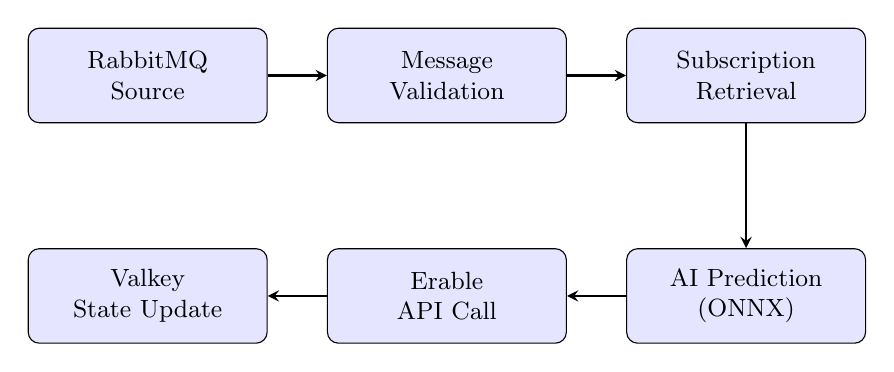
\begin{tikzpicture}[
        node distance=1.8cm,
        block/.style={rectangle, draw, fill=blue!10, text width=2.8cm, text centered, minimum height=1.2cm, rounded corners, font=\small},
        arrow/.style={->, >=stealth, thick}
    ]
        \node[block] (src) {RabbitMQ\\Source};
        \node[block, right of=src, xshift=2cm] (valid) {Message\\Validation};
        \node[block, right of=valid, xshift=2cm] (sub) {Subscription\\Retrieval};
        \node[block, below of=sub, yshift=-1cm] (ai) {AI Prediction\\(ONNX)};
        \node[block, left of=ai, xshift=-2cm] (erable) {Erable\\API Call};
        \node[block, left of=erable, xshift=-2cm] (sink) {Valkey\\State Update};

        \draw[arrow] (src) -- (valid);
        \draw[arrow] (valid) -- (sub);
        \draw[arrow] (sub) -- (ai);
        \draw[arrow] (ai) -- (erable);
        \draw[arrow] (erable) -- (sink);
    \end{tikzpicture}
    \caption{LFU job logical pipeline}
    \label{fig:logical-pipeline}
\end{figure}

\subsection{Erable API Call Operator}

The \texttt{LFUErableCallProcessFunction} sends the push notification to the Erable system via an HTTP POST call. It:
\begin{enumerate}
    \item Builds the \texttt{LFUErableEntity} containing the MSISDN, customer type, event type, and reached threshold.
    \item Sends the request via Spring \texttt{WebClient} with a configurable retry mechanism.
    \item Only forwards the message downstream if the response is \texttt{2xx}.
    \item Increments per-SID counters (OMOI, SOSH, OPRO) for successful sends.
\end{enumerate}

\begin{lstlisting}[language=Java, caption={HTTP call to Erable}]
LFUErableEntity body = buildEntity(fairUseMessage);
String erableUri = ErableCallUtils.getPath(
    erableCallConfiguration.getErableHost(),
    erableCallConfiguration.getErablePathPattern(), sid);

ResponseEntity<String> response = ErableCallUtils.sendErableRequest(
    client, erableUri, erableUuid, body,
    erableCallConfiguration, LOG);

if (response.getStatusCode().is2xxSuccessful()) {
    incrementOmoiOrSoshOrOpro(/* counters */);
    collector.collect(notification);
}
\end{lstlisting}

\subsection{Erable Error Handling}

\begin{itemize}
    \item \textbf{Automatic retry} via \texttt{ErableCallUtils.shouldRetry()} for transient errors (connection timeouts, 5xx responses).
    \item \textbf{Critical errors} (e.g., repeated 5xx): exception propagation via \texttt{throwIfCriticalStatus()} to trigger a Flink restart.
    \item \textbf{Non-critical errors} (e.g., 4xx): log with code \texttt{UNMANAGED\_ERROR} + counter increment, message dropped.
    \item \textbf{Null response}: logged as \texttt{ERABLE\_ACCESS\_ERROR}, message dropped.
\end{itemize}

\subsection{State Update Sink}

The \texttt{LFUUpdateSubscriptionSink} class updates the \texttt{LfuMainRecord}'s state in Valkey with the timestamp of the last processed event. This enables the next processing cycle to compute the time interval since the last notification.

\begin{lstlisting}[language=Java, caption={State update in Valkey}]
lfuMainRecord.getState().setStates(
    Map.of(eventType, Map.of("last", timestamp)));
dao.updateLfuMainRecord(lfuMainRecord);
\end{lstlisting}

\texttt{DataPersistenceException} errors are caught, logged with code \texttt{PERSISTENCE\_LIB\_ACCESS\_ERROR}, and the per-SID failed counter is incremented.

\subsection{Sprint 3 Outcome}

At the end of Sprint~3, the full notification pipeline was functional end-to-end: messages were consumed from RabbitMQ, validated, enriched with subscription data, sent to Erable, and their state persisted in Valkey. The stub mode (\texttt{ERABLE\_STUBBED=true}) allowed testing without a live Erable instance.

%######################################################################
%######################################################################
\section{Sprint 4: AI Prediction Module}
\label{sec:sprint4}
%######################################################################
%######################################################################

\subsection{Sprint Goal}

Integrate an AI prediction layer into the pipeline to predict quota overshoot probability and detect anomalous consumption patterns, without disrupting the existing notification flow.

\subsection{Overview}

The AI prediction step is implemented in \texttt{LFUPredictionProcessFunction}. It predicts in real time:
\begin{itemize}
    \item The \textbf{probability of quota overshoot} (\texttt{predictionScore} $\in [0, 1]$)
    \item Whether the \textbf{consumption pattern is anomalous} (\texttt{anomalyDetected} if score $\geq$ threshold)
\end{itemize}

\subsection{Dataset}

The model is trained on historical fair-use notification data collected from the production pipeline.

\paragraph{Data Sources}
\begin{itemize}
    \item \textbf{FairUse events} (RabbitMQ): MSISDN, customer type, event type, reached threshold, date.
    \item \textbf{Subscription state} (Valkey): timestamp of the last notification per event type.
\end{itemize}

Each sample is labeled according to whether a quota overshoot actually occurred within the billing cycle (binary label: overshoot / no overshoot).

\subsection{Feature Extraction}

The \texttt{PredictionFeatureExtractor} class extracts \textbf{7 features} normalized to the $[0, 1]$ range:

\begin{table}[H]
    \centering
    \caption{Model feature description}
    \label{tab:features}
    \begin{tabularx}{\textwidth}{c l l X}
\toprule
\textbf{\#} & \textbf{Feature} & \textbf{Encoding} & \textbf{Rationale} \\
\midrule
1 & Reached Threshold (\%) & $\frac{\text{value}}{100}$ &
Direct indicator of quota consumption level. \\
\addlinespace
2 & Customer Type & GP$=$0, ENT$=$0.5, MVNO$=$1 &
Segments with distinct consumption profiles. \\
\addlinespace
3 & Hour of Day & $\frac{\text{hour}}{23}$ &
Intra-day consumption patterns (peak hours). TZ: Europe/Paris. \\
\addlinespace
4 & Day of Week & $\frac{\text{day} - 1}{6}$ &
Weekly seasonality (weekday vs.\ weekend). \\
\addlinespace
5 & Hours Since Last Notif. & $\frac{\text{hours}}{720}$ (capped at 30d) &
Notification recency. Short interval = rapid consumption. \\
\addlinespace
6 & Day in Billing Cycle & $\frac{\text{dayOfMonth} - 1}{\text{daysInMonth} - 1}$ &
\textbf{Critical feature}: 80\% on day~5 is far more alarming than on day~28 (billing resets on the 1\textsuperscript{st}). \\
\addlinespace
7 & Event Type & fairuse$=$0, blocage$=$0.25, redirect$=$0.5, alerting$=$0.75, leveeFU$=$1 &
Event severity. Blocking/redirect = higher risk. \\
\bottomrule
    \end{tabularx}
\end{table}

\begin{lstlisting}[language=Java, caption={Feature extraction (PredictionFeatureExtractor.java)}]
public float[] extractFeatures(EnrichedFairUseMessage message) {
    float[] features = new float[FEATURE_COUNT]; // 7 features
    features[0] = fairuse.getReachedThresholdPercent() / 100.0f;
    features[1] = encodeCustomerType(fairuse.getCustomerType());
    features[2] = eventTime.getHour() / 23.0f;
    features[3] = (eventTime.getDayOfWeek().getValue() - 1) / 6.0f;
    features[4] = computeHoursSinceLastNotification(mainRecord, fairuse);
    features[5] = computeDayInBillingCycle(eventTime);
    features[6] = encodeEventType(fairuse.getEventType());
    return features;
}
\end{lstlisting}

\subsection{Prediction Model}

\subsubsection{Algorithm}

The model is a \textbf{binary classifier} exported in \textbf{ONNX format} (\textit{Open Neural Network Exchange}), loaded at runtime via the ONNX Runtime Java API (\texttt{com.microsoft.onnxruntime:1.17.0}).

The recommended algorithm is a \textbf{Gradient Boosted Decision Tree (GBDT)} such as XGBoost or LightGBM, chosen for:
\begin{itemize}
    \item Excellent performance on low-dimensional tabular data (7~features);
    \item High interpretability (feature importance analysis);
    \item Very low inference latency ($< 1$~ms), compatible with stream processing;
    \item ONNX format enabling training in Python and native JVM deployment.
\end{itemize}

\subsubsection{ONNX Inference}

\begin{lstlisting}[language=Java, caption={ONNX inference in the Flink pipeline}]
private double runOnnxInference(float[] features) throws OrtException {
    long[] shape = {1, PredictionFeatureExtractor.FEATURE_COUNT};
    FloatBuffer buffer = FloatBuffer.wrap(features);
    OnnxTensor inputTensor = OnnxTensor.createTensor(
        ortEnvironment, buffer, shape);
    try (Result result = ortSession.run(
            Collections.singletonMap("input", inputTensor))) {
        float[][] output = (float[][]) result.get(0).getValue();
        return output[0][0]; // Overshoot probability
    } finally {
        inputTensor.close();
    }
}
\end{lstlisting}

\subsubsection{Rule-Based Fallback}

A \textbf{fallback algorithm} is automatically activated when the ONNX model is unavailable. It combines 4 weighted factors:

\begin{equation}
    \label{eq:fallback}
    \text{score} = 0.35 \times \underbrace{\text{thresholdRisk}}_{f_1}
    + 0.25 \times \underbrace{f_1 \times (1 - f_6)}_{\text{urgencyFactor}}
    + 0.20 \times \underbrace{(1 - f_5)}_{\text{recencyRisk}}
    + 0.20 \times \underbrace{f_7}_{\text{eventRisk}}
\end{equation}

The key insight encoded is: high quota usage early in the billing cycle is exponentially more critical than the same usage near the end. For example:
\begin{itemize}
    \item 80\% on day~3 ($f_6 \approx 0.07$) $\Rightarrow$ urgencyFactor $\approx 0.80 \times 0.93 = 0.74$ (high urgency)
    \item 80\% on day~28 ($f_6 \approx 0.90$) $\Rightarrow$ urgencyFactor $\approx 0.80 \times 0.10 = 0.08$ (low urgency)
\end{itemize}

\subsubsection{Training Pipeline}

Training is performed offline in Python following these steps:

\begin{enumerate}
    \item \textbf{Data collection}: Extraction of historical events and their outcomes (overshoot within the billing cycle).
    \item \textbf{Feature engineering}: Exact reproduction of the 7~features from \texttt{PredictionFeatureExtractor} to ensure training/inference consistency.
    \item \textbf{Partitioning}: Stratified split 70\%~/~15\%~/~15\% (train / validation / test).
    \item \textbf{Hyperparameter tuning}: Bayesian optimization over key parameters (\texttt{max\_depth}, \texttt{learning\_rate}, \texttt{n\_estimators}, \texttt{min\_child\_weight}).
    \item \textbf{Export}: Conversion to ONNX via \texttt{skl2onnx} or \texttt{onnxmltools}, then integration into the Docker container at \texttt{/models/fairuse\_prediction.onnx}.
\end{enumerate}

\subsubsection{Evaluation Metrics}

\begin{table}[H]
    \centering
    \caption{Model evaluation metrics and targets}
    \label{tab:metrics}
    \begin{tabularx}{\textwidth}{l X c}
\toprule
\textbf{Metric} & \textbf{Description} & \textbf{Target} \\
\midrule
Accuracy &
Proportion of correct predictions on the test set. &
$\geq 90\%$ \\
\addlinespace
Precision &
$\frac{TP}{TP + FP}$. Proportion of predicted overshoots that are real.
High precision avoids unnecessary customer notifications. &
$\geq 85\%$ \\
\addlinespace
Recall &
$\frac{TP}{TP + FN}$. Proportion of actual overshoots detected.
High recall ensures no customer is surprised by unexpected quota exhaustion. &
$\geq 80\%$ \\
\addlinespace
F1-Score &
Harmonic mean: $\frac{2 \times P \times R}{P + R}$.
Balances false alarms and missed detections. &
$\geq 82\%$ \\
\addlinespace
RMSE &
Root Mean Squared Error on the prediction score $[0, 1]$.
Measures calibration (predicted probability vs.\ actual overshoot frequency). &
$\leq 0.15$ \\
\addlinespace
AUC-ROC &
Area Under the ROC Curve. Discrimination ability across all thresholds. &
$\geq 0.92$ \\
\bottomrule
    \end{tabularx}
\end{table}

\subsection{Resilience Design}

The AI prediction step is designed to be \textbf{non-blocking}:
\begin{itemize}
    \item If the ONNX model cannot be loaded $\Rightarrow$ automatic activation of the rule-based fallback.
    \item If inference fails at runtime $\Rightarrow$ the message is forwarded with \texttt{predictionScore = -1.0}.
    \item The notification pipeline is \textbf{never interrupted} by an AI issue.
\end{itemize}

\subsection{Sprint 4 Outcome}

At the end of Sprint~4, every message flowing through the pipeline was enriched with an AI prediction score. The fallback mechanism was validated by running tests without the ONNX model file present, confirming zero impact on the notification flow.

%######################################################################
%######################################################################
\section{Sprint 5: Containerization and Deployment}
\label{sec:sprint5}
%######################################################################
%######################################################################

\subsection{Sprint Goal}

Package the LFU job as a production-ready Docker image, configure high-availability deployment, and establish Flink checkpointing for fault tolerance.

\subsection{Physical Architecture}

\begin{figure}[H]
    \centering
    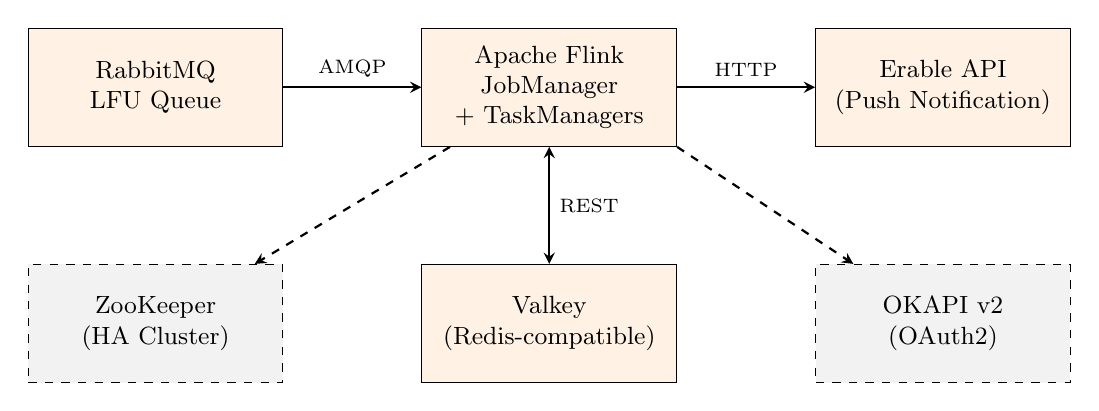
\begin{tikzpicture}[
        node distance=2cm,
        component/.style={rectangle, draw, fill=orange!10, text width=3cm, text centered, minimum height=1.5cm, font=\small},
        infra/.style={rectangle, draw, fill=gray!10, text width=3cm, text centered, minimum height=1.5cm, font=\small, dashed},
        arrow/.style={->, >=stealth, thick}
    ]
% Row 1
        \node[component] (rmq) {RabbitMQ\\LFU Queue};
        \node[component, right of=rmq, xshift=3cm] (flink) {Apache Flink\\JobManager\\+ TaskManagers};
        \node[component, right of=flink, xshift=3cm] (erable) {Erable API\\(Push Notification)};

% Row 2
        \node[infra, below of=rmq, yshift=-1cm] (zk) {ZooKeeper\\(HA Cluster)};
        \node[component, below of=flink, yshift=-1cm] (valkey) {Valkey\\(Redis-compatible)};
        \node[infra, below of=erable, yshift=-1cm] (okapi) {OKAPI v2\\(OAuth2)};

% Arrows
        \draw[arrow] (rmq) -- node[above, font=\scriptsize]{AMQP} (flink);
        \draw[arrow] (flink) -- node[above, font=\scriptsize]{HTTP} (erable);
        \draw[arrow, <->] (flink) -- node[right, font=\scriptsize]{REST} (valkey);
        \draw[arrow, dashed] (flink) -- (zk);
        \draw[arrow, dashed] (flink.south east) -- (okapi);
    \end{tikzpicture}
    \caption{LFU job physical architecture}
    \label{fig:physical-arch}
\end{figure}

\subsection{Docker Image}

The job is packaged in a Docker image based on a customized Flink base image. The \texttt{maven-shade-plugin} produces a fat JAR containing all dependencies (including ONNX Runtime and the embedded AI model).

\begin{lstlisting}[language=bash, caption={Dockerfile (excerpt)}]
FROM pfs-notif-docker.artifactory.../flink_base:1.20.1_scala_2.12_FIX

# Hebex CA certificates for internal APIs (Valkey, Erable, OKAPI)
RUN apt-get install -y hebex-ca-certificates

# Flink dependencies (logback, jackson, slf4j)
COPY flink-dependencies/*logback*.jar $FLINK_HOME/lib/
COPY flink-dependencies/jackson*.jar $FLINK_HOME/lib/
COPY flink-dependencies/slf4j-api-*.jar $FLINK_HOME/lib/

# LFU job fat JAR (including ONNX model in resources)
COPY $job_jar_name $FLINK_HOME/usrlib

# Timezone Europe/Paris for correct log timestamps
RUN ln -snf /usr/share/zoneinfo/Europe/Paris /etc/localtime

# Import Scality S3 certificate into Java keystore
RUN keytool -import -alias ca-s3 \
    -keystore $JAVA_HOME/lib/security/cacerts \
    -file /usr/lib/ssl/certs/root_sha512.pki_orange.pem \
    -storepass changeit -noprompt
\end{lstlisting}

\subsection{Flink Cluster Configuration}

The production deployment uses a high-availability architecture:

\begin{itemize}
    \item \textbf{2 JobManagers} in active/passive mode, coordinated via ZooKeeper (3 nodes).
    \item \textbf{3+ TaskManagers} with 2 task slots each (configurable via \texttt{TASK\_MANAGER\_NUMBER\_OF\_TASK\_SLOTS}).
    \item \textbf{Checkpoints} stored on the shared filesystem (\texttt{/opt/flink/checkpoints}).
    \item \textbf{HA metadata} stored in ZooKeeper and the local filesystem (\texttt{/opt/flink/flink-ha}).
\end{itemize}

\subsection{Checkpointing and Fault Tolerance}

\begin{lstlisting}[language=Java, caption={Checkpoint configuration (LFUJob.java)}]
if (CHECKPOINT_ENABLED) {
    env.enableCheckpointing(
        Long.parseLong(CHECKPOINT_INTERVAL_IN_MS), CHECKPOINTING_MODE);
    env.getCheckpointConfig()
       .setMinPauseBetweenCheckpoints(MIN_PAUSE_BETWEEN_CHECKPOINTS);
    env.getCheckpointConfig()
       .setCheckpointTimeout(CHECKPOINT_TIMEOUT_IN_MS);
    env.getCheckpointConfig()
       .setMaxConcurrentCheckpoints(MAX_CONCURRENT_CHECKPOINTS);
    env.getCheckpointConfig()
       .setExternalizedCheckpointCleanup(EXTERNALIZED_CHECKPOINT_CLEANUP);
}
\end{lstlisting}

\begin{itemize}
    \item \textbf{Mode}: \texttt{EXACTLY\_ONCE} (default) or \texttt{AT\_LEAST\_ONCE} (required for correlation ID).
    \item \textbf{Interval}: Configurable (default 1000~ms in dev, 10000~ms in integration).
    \item \textbf{Externalized checkpoints}: Retained after job cancellation to allow restart from the last consistent state.
    \item \textbf{Compression}: Optional snapshot compression to reduce storage overhead.
\end{itemize}

\subsection{Rebalance Strategy}

Each operator is followed by a \texttt{.rebalance()}, ensuring round-robin distribution of the stream across parallel instances. This avoids \textit{hot spots} when certain MSISDNs generate disproportionately more events than others.

\subsection{Environment Variables}

\begin{table}[H]
    \centering
    \caption{Main environment variables}
    \label{tab:env-vars}
    \begin{tabularx}{\textwidth}{l c X}
\toprule
\textbf{Variable} & \textbf{Default} & \textbf{Description} \\
\midrule
\multicolumn{3}{l}{\textit{RabbitMQ Source}} \\
\texttt{RMQ\_LFU\_QUEUE} & --- & RabbitMQ queue name \\
\texttt{RMQ\_HOST} & --- & RabbitMQ broker host \\
\texttt{USE\_CORRELATION\_ID} & false & Enable correlation ID tracking \\
\midrule
\multicolumn{3}{l}{\textit{Flink}} \\
\texttt{GLOBAL\_PARALLELISM} & 1 & Global job parallelism \\
\texttt{CHECKPOINT\_ENABLED} & false & Enable checkpointing \\
\texttt{CHECKPOINT\_INTERVAL\_IN\_MS} & 1000 & Interval between checkpoints (ms) \\
\texttt{CHECKPOINT\_MODE} & EXACTLY\_ONCE & Checkpointing mode \\
\texttt{USE\_SNAPSHOT\_COMPRESSION} & false & Snapshot compression \\
\texttt{LATENCY\_INTERVAL} & --- & Latency tracking interval \\
\midrule
\multicolumn{3}{l}{\textit{Valkey}} \\
\texttt{VALKEY\_HOST\_HTTP} & --- & Valkey API URL \\
\texttt{VALKEY\_BASE\_PATH} & /pns/v3/users & API base path \\
\midrule
\multicolumn{3}{l}{\textit{Erable}} \\
\texttt{ERABLE\_HOST} & --- & Erable service URL \\
\texttt{ERABLE\_STUBBED} & false & Stub mode (testing) \\
\midrule
\multicolumn{3}{l}{\textit{Artificial Intelligence}} \\
\texttt{AI\_ANOMALY\_THRESHOLD} & 0.85 & Anomaly detection threshold \\
\texttt{AI\_MODEL\_PATH} & /models/fairuse\_prediction.onnx & ONNX model path \\
\bottomrule
    \end{tabularx}
\end{table}

\subsection{Sprint 5 Outcome}

At the end of Sprint~5, the LFU job was deployable as a Docker container on Kubernetes with full high-availability support. The CI/CD pipeline produced the fat JAR, built the Docker image, and pushed it to the Artifactory registry. Checkpoint recovery was validated by simulating TaskManager failures.

%######################################################################
%######################################################################
\section{Sprint 6: Observability and Monitoring}
\label{sec:sprint6}
%######################################################################
%######################################################################

\subsection{Sprint Goal}

Implement comprehensive observability through structured logging (Kibana), real-time metrics dashboards (Grafana), and alerting rules to ensure production-grade monitoring.

\subsection{Structured Logging}

\subsubsection{Log Architecture}

All log entries are structured as JSON using the \texttt{Logstash Logback Encoder}, enabling machine-parseable logs that are ingested into an \textbf{ELK stack} (Elasticsearch, Logstash, Kibana). Each log entry contains structured markers via \texttt{net.logstash.logback.marker.Markers.appendEntries()}.

\subsubsection{Log Keys}

Every log entry is enriched with the following structured fields, defined in \texttt{LogKeys}:

\begin{table}[H]
    \centering
    \caption{Structured log fields}
    \label{tab:log-keys}
    \begin{tabularx}{\textwidth}{l l X}
\toprule
\textbf{Field} & \textbf{Key} & \textbf{Description} \\
\midrule
\texttt{customCode} & \texttt{customCode} & Numeric code identifying the log event category (see Table~\ref{tab:log-codes}) \\
\texttt{uuid} & \texttt{uuid} & Unique message traceability identifier \\
\texttt{topologyName} & \texttt{topologyName} & Job name (\texttt{LFU}) \\
\texttt{sid} & \texttt{sid} & Service ID (OMOI, SOSH, OPRO) \\
\texttt{msisdn} & \texttt{msisdn} & Customer phone number \\
\texttt{X-ERABLE-uuid} & \texttt{X-ERABLE-uuid} & Erable request correlation UUID \\
\bottomrule
    \end{tabularx}
\end{table}

\subsubsection{Log Code Classification}

The \texttt{CodeMessageLog} enum provides a standardized classification for all log events:

\begin{table}[H]
    \centering
    \caption{Log code classification (\texttt{CodeMessageLog})}
    \label{tab:log-codes}
    \begin{tabularx}{\textwidth}{l l l X}
\toprule
\textbf{Code} & \textbf{Level} & \textbf{Constant} & \textbf{Message} \\
\midrule
\multicolumn{4}{l}{\textit{Informational (0xxx--1xxx)}} \\
0000 & DEBUG & \texttt{INFORMATIONAL\_MESSAGE} & Informational message \\
1000 & INFO & \texttt{NOTIFICATION\_PROCESS\_COMPLETED} & Notification process completed \\
\midrule
\multicolumn{4}{l}{\textit{Success (2xxx)}} \\
2000 & DEBUG & \texttt{ERABLE\_SEND\_SUCCESSFULLY} & Notification sent to Erable successfully \\
\midrule
\multicolumn{4}{l}{\textit{Discarded (2xxx)}} \\
2041 & INFO & \texttt{NOTIFICATION\_DISCARDED} & Notification discarded \\
2045 & WARN & \texttt{UNMANAGED\_EVENT} & Unmanaged event type for notif \\
2047 & INFO & \texttt{NO\_MAIN\_RECORD\_FOR\_NOTIF} & No main record for notif \\
\midrule
\multicolumn{4}{l}{\textit{Client Errors (4xxx)}} \\
4000 & ERROR & \texttt{MISSING\_MANDATORY\_PARAMETERS} & Missing mandatory parameters \\
4150 & ERROR & \texttt{NOT\_VALID\_JSON} & Not valid JSON \\
4401 & ERROR & \texttt{NO\_DATA} & No data \\
\midrule
\multicolumn{4}{l}{\textit{System Errors (5xxx)}} \\
5030 & ERROR & \texttt{ERABLE\_ACCESS\_ERROR} & Erable access error \\
5031 & ERROR & \texttt{PERSISTENCE\_LIB\_ACCESS\_ERROR} & Valkey access error \\
5036 & ERROR & \texttt{UNMANAGED\_ERROR} & Unmanaged error \\
\bottomrule
    \end{tabularx}
\end{table}

\subsubsection{Log Example}

A typical structured log entry produced by the LFU job:

\begin{lstlisting}[caption={Structured JSON log entry example}]
{
  "timestamp": "2026-06-30T14:32:15.123+02:00",
  "level": "INFO",
  "logger": "LFUGetSubscriptionProcessFunction",
  "message": "Processing notification, main record found: ...",
  "customCode": "0000",
  "uuid": "a1b2c3d4-e5f6-7890-abcd-ef1234567890",
  "topologyName": "LFU",
  "sid": "omoi",
  "msisdn": "33612345678"
}
\end{lstlisting}

\subsection{Kibana Dashboards}

The structured logs are ingested into Elasticsearch and visualized through Kibana dashboards. Figure~\ref{fig:kibana-logs} shows the main log exploration view, and Figure~\ref{fig:kibana-errors} shows the error monitoring dashboard.

\begin{figure}[H]
    \centering
    \fbox{\parbox{0.9\textwidth}{\centering\vspace{2cm}
    \textit{[Screenshot: Kibana Discover view showing LFU job structured logs filtered by \texttt{topologyName:LFU}. Visible columns: timestamp, level, customCode, uuid, msisdn, sid, message.]}
    \vspace{2cm}}}
    \caption{Kibana --- LFU job log exploration view}
    \label{fig:kibana-logs}
\end{figure}

\begin{figure}[H]
    \centering
    \fbox{\parbox{0.9\textwidth}{\centering\vspace{2cm}
    \textit{[Screenshot: Kibana dashboard showing error distribution by customCode. Bar chart of error codes (5030, 5031, 5036, 4000, 4150) over time. Pie chart showing error proportions per SID (OMOI, SOSH, OPRO).]}
    \vspace{2cm}}}
    \caption{Kibana --- LFU error monitoring dashboard}
    \label{fig:kibana-errors}
\end{figure}

Key Kibana queries used for monitoring:

\begin{table}[H]
    \centering
    \caption{Kibana queries for LFU monitoring}
    \label{tab:kibana-queries}
    \begin{tabularx}{\textwidth}{l X}
\toprule
\textbf{Purpose} & \textbf{KQL Query} \\
\midrule
All LFU logs & \texttt{topologyName:"LFU"} \\
Errors only & \texttt{topologyName:"LFU" AND level:"ERROR"} \\
Erable failures & \texttt{topologyName:"LFU" AND customCode:"5030"} \\
Valkey failures & \texttt{topologyName:"LFU" AND customCode:"5031"} \\
Discarded messages & \texttt{topologyName:"LFU" AND customCode:"2041"} \\
Successful deliveries & \texttt{topologyName:"LFU" AND customCode:"2000"} \\
Completed notifications & \texttt{topologyName:"LFU" AND customCode:"1000"} \\
Track specific customer & \texttt{topologyName:"LFU" AND msisdn:"33612345678"} \\
Trace by UUID & \texttt{uuid:"a1b2c3d4-..."} \\
AI anomalies & \texttt{topologyName:"LFU" AND message:"Anomaly detected"} \\
\bottomrule
    \end{tabularx}
\end{table}

\subsection{Flink Metrics}

Each operator exposes counters via the Flink metrics system. These are scraped by \textbf{Prometheus} (port 9249) and visualized in \textbf{Grafana}.

\begin{table}[H]
    \centering
    \caption{Metrics exposed by the LFU job}
    \label{tab:runtime-metrics}
    \begin{tabularx}{\textwidth}{l l X}
\toprule
\textbf{Metric} & \textbf{Operator} & \textbf{Description} \\
\midrule
\texttt{incoming\_requests} & Validation & Total number of messages received \\
\texttt{discarded\_requests} & Validation, Subscription & Messages rejected (invalid or no main record) \\
\texttt{failed\_requests} & Subscription, Erable, Sink & Valkey or Erable access errors \\
\texttt{sent\_requests\_omoi} & Erable & Notifications sent for Orange et Moi \\
\texttt{sent\_requests\_sosh} & Erable & Notifications sent for My Sosh \\
\texttt{sent\_requests\_opro} & Erable & Notifications sent for Orange Pro \\
\texttt{predictions\_total} & AI & Total number of predictions performed \\
\texttt{anomalies\_detected} & AI & Consumption anomalies detected \\
\texttt{fallback\_used} & AI & Predictions using rule-based fallback \\
\bottomrule
    \end{tabularx}
\end{table}

\subsection{Grafana Dashboards}

Four Grafana dashboards were created for comprehensive LFU monitoring.

\subsubsection{Dashboard 1: Pipeline Overview}

\begin{figure}[H]
    \centering
    \fbox{\parbox{0.9\textwidth}{\centering\vspace{2cm}
    \textit{[Screenshot: Grafana dashboard ``LFU Pipeline Overview''. Panels include: (1)~incoming\_requests rate (messages/sec), (2)~discarded\_requests rate, (3)~sent\_requests total by SID (stacked bar: OMOI in orange, SOSH in green, OPRO in blue), (4)~pipeline throughput gauge.]}
    \vspace{2cm}}}
    \caption{Grafana --- LFU pipeline overview dashboard}
    \label{fig:grafana-overview}
\end{figure}

Key PromQL queries for this dashboard:

\begin{lstlisting}[caption={PromQL queries for pipeline overview}]
# Incoming message rate (messages/sec)
rate(flink_taskmanager_job_task_operator_incoming_requests[5m])

# Discarded message rate
rate(flink_taskmanager_job_task_operator_discarded_requests[5m])

# Sent requests by SID
sum by (client) (
  rate(flink_taskmanager_job_task_operator_sent_requests[5m])
)
\end{lstlisting}

\subsubsection{Dashboard 2: Error Monitoring}

\begin{figure}[H]
    \centering
    \fbox{\parbox{0.9\textwidth}{\centering\vspace{2cm}
    \textit{[Screenshot: Grafana dashboard ``LFU Errors''. Panels include: (1)~failed\_requests rate by SID, (2)~Erable error rate vs.\ success rate, (3)~Valkey error rate, (4)~error ratio alert (red threshold line at 5\%).]}
    \vspace{2cm}}}
    \caption{Grafana --- LFU error monitoring dashboard}
    \label{fig:grafana-errors}
\end{figure}

\begin{lstlisting}[caption={PromQL queries for error monitoring}]
# Failed requests rate by SID
sum by (client) (
  rate(flink_taskmanager_job_task_operator_failed_requests[5m])
)

# Error ratio (alert if > 5%)
sum(rate(flink_taskmanager_job_task_operator_failed_requests[5m]))
/
sum(rate(flink_taskmanager_job_task_operator_incoming_requests[5m]))
\end{lstlisting}

\subsubsection{Dashboard 3: AI Prediction Monitoring}

\begin{figure}[H]
    \centering
    \fbox{\parbox{0.9\textwidth}{\centering\vspace{2cm}
    \textit{[Screenshot: Grafana dashboard ``LFU AI Predictions''. Panels include: (1)~predictions\_total rate, (2)~anomalies\_detected rate with threshold line, (3)~anomaly ratio (anomalies/predictions), (4)~fallback\_used counter (should be 0 in normal operation).]}
    \vspace{2cm}}}
    \caption{Grafana --- LFU AI prediction monitoring dashboard}
    \label{fig:grafana-ai}
\end{figure}

\begin{lstlisting}[caption={PromQL queries for AI monitoring}]
# Prediction rate
rate(flink_taskmanager_job_task_operator_predictions_total[5m])

# Anomaly detection rate
rate(flink_taskmanager_job_task_operator_anomalies_detected[5m])

# Anomaly ratio
rate(flink_taskmanager_job_task_operator_anomalies_detected[5m])
/
rate(flink_taskmanager_job_task_operator_predictions_total[5m])

# Fallback usage (alert if > 0)
flink_taskmanager_job_task_operator_fallback_used
\end{lstlisting}

\subsubsection{Dashboard 4: Flink Cluster Health}

\begin{figure}[H]
    \centering
    \fbox{\parbox{0.9\textwidth}{\centering\vspace{2cm}
    \textit{[Screenshot: Grafana dashboard ``Flink Cluster Health''. Panels include: (1)~number of running TaskManagers, (2)~checkpoint duration (ms), (3)~checkpoint size (bytes), (4)~latency tracking per operator, (5)~JVM heap usage per TaskManager.]}
    \vspace{2cm}}}
    \caption{Grafana --- Flink cluster health dashboard}
    \label{fig:grafana-cluster}
\end{figure}

\subsection{Alerting Rules}

The following Prometheus alerting rules are configured to trigger PagerDuty/email notifications:

\begin{table}[H]
    \centering
    \caption{Prometheus alerting rules}
    \label{tab:alerts}
    \begin{tabularx}{\textwidth}{l l X}
\toprule
\textbf{Alert Name} & \textbf{Condition} & \textbf{Description} \\
\midrule
\texttt{LFUHighErrorRate} & Error ratio $> 5\%$ for 5~min & Too many messages failing \\
\texttt{LFUErableDown} & Erable failures $> 10$/min for 5~min & Erable API unreachable \\
\texttt{LFUValkeyDown} & Valkey failures $> 10$/min for 5~min & Valkey state store unreachable \\
\texttt{LFUAIFallbackActive} & \texttt{fallback\_used} $> 0$ for 10~min & ONNX model not loaded \\
\texttt{LFUHighAnomalyRate} & Anomaly ratio $> 20\%$ for 15~min & Unusual consumption patterns \\
\texttt{LFUNoIncoming} & \texttt{incoming\_requests} $= 0$ for 10~min & No messages received \\
\texttt{LFUCheckpointFailing} & Checkpoint failures $> 3$ & State consistency at risk \\
\bottomrule
    \end{tabularx}
\end{table}

\subsection{End-to-End Traceability}

A single notification can be traced through the entire system using the \texttt{uuid} field:

\begin{enumerate}
    \item \textbf{Kibana}: Search by \texttt{uuid} to see every log entry for a specific message, from ingestion through delivery.
    \item \textbf{Grafana}: Correlate timestamps from Kibana with metric spikes (e.g., an error burst at 14:32 matching an Erable outage).
    \item \textbf{Erable}: The \texttt{X-ERABLE-uuid} field allows tracing the notification into the downstream push notification system.
\end{enumerate}

\begin{figure}[H]
    \centering
    \fbox{\parbox{0.9\textwidth}{\centering\vspace{2cm}
    \textit{[Screenshot: Kibana Discover filtered by a single UUID, showing 5 log entries tracing a message through: (1)~``Received notification'' (code 0000), (2)~``Processing notification, main record found'' (code 0000), (3)~``Anomaly detected'' (AI prediction), (4)~``Notification sent to Erable successfully'' (code 2000), (5)~``Notification process completed'' (code 1000).]}
    \vspace{2cm}}}
    \caption{Kibana --- End-to-end message traceability by UUID}
    \label{fig:kibana-trace}
\end{figure}

\subsection{Sprint 6 Outcome}

At the end of Sprint~6, the LFU job had complete production observability. Operators could monitor the system in real time through Grafana dashboards and investigate specific issues through Kibana log search. Alerting rules provided proactive notification of system degradation.

%######################################################################
%######################################################################
\section{Testing}
\label{sec:testing}
%######################################################################
%######################################################################

The job is covered across all sprints by:
\begin{itemize}
    \item \textbf{Unit tests}: Each operator is tested in isolation with mocks (Mockito 4.5.1) for Valkey and Erable. Log assertions validate that correct \texttt{CodeMessageLog} entries are emitted using the shared \texttt{LogAssertionUtils}.
    \item \textbf{Integration tests}: Full pipeline validation with a local Flink environment and mocked external services.
    \item \textbf{End-to-end tests}: Message publication to local RabbitMQ and verification of the Valkey state output.
\end{itemize}

The \texttt{pushavoo-flink-test} module provides shared test utilities across all jobs, including \texttt{LogAppender} for capturing and asserting structured log output.

%######################################################################
%######################################################################
\section{Summary}
\label{sec:implementation-summary}
%######################################################################
%######################################################################

Over 6 sprints, the LFU job was developed incrementally from a simple message consumer to a fully observable, AI-enhanced notification pipeline:

\begin{enumerate}
    \item \textbf{Sprint 1}: Project foundation --- RabbitMQ ingestion and message validation.
    \item \textbf{Sprint 2}: Business logic --- Valkey subscription retrieval and rule validation.
    \item \textbf{Sprint 3}: Core delivery --- Erable notification sending and state persistence.
    \item \textbf{Sprint 4}: Intelligence --- ONNX-based AI prediction with rule-based fallback.
    \item \textbf{Sprint 5}: Production readiness --- Docker containerization, Kubernetes deployment, checkpointing.
    \item \textbf{Sprint 6}: Observability --- Structured logging (Kibana), metrics dashboards (Grafana), alerting.
\end{enumerate}

This architecture enables the processing of fair-use events with minimal latency while guaranteeing the reliability of the push notification system for millions of Orange customers.

